%% ==================
\chapter{Results}
\label{ch:results}
%% ==================
%
%My results:

\section{Recreating previous results}
%	-Only 3 original components
%		-Spherical excess
%		-very bad chi2 in disk and bubbles

Introduce the weniger plots here (or in the state of the research?) to show excess in GC.
\begin{figure}[h]
  \centering
  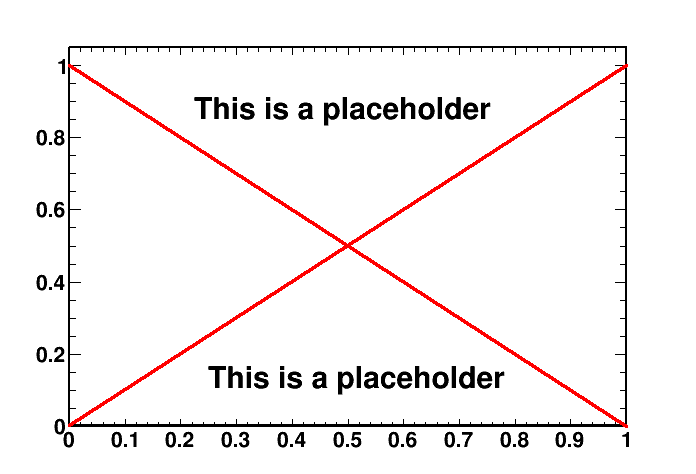
\includegraphics[width=.9\linewidth]{pic/dummy.png}
  \caption{Some weniger plots to show the GC excess}
  \label{fig:weniger_plot}
\end{figure}



\begin{figure}[h]
  \centering
  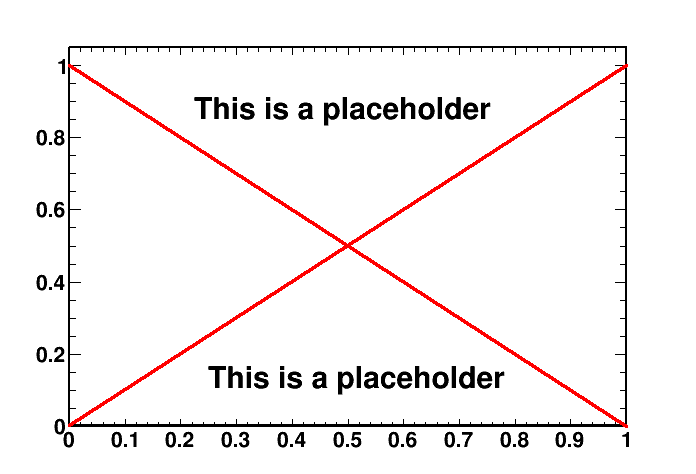
\includegraphics[width=.9\linewidth]{pic/dummy.png}
  \caption{Picture of GC excess, (compare with previous papers?), a chi2 map too}
  \label{fig:original_GC_excess}
\end{figure}

Before trying upgrade the model in use, it is important to make sure we can recreate it with the same parameters. Fig. \ref{fig:original_GC_excess} shows the results of a fit using only the PCR, IC and BR components. The shape and intensity of the previously observed excess are found \todo{cite}.\\

\begin{figure}[h]
  \centering
  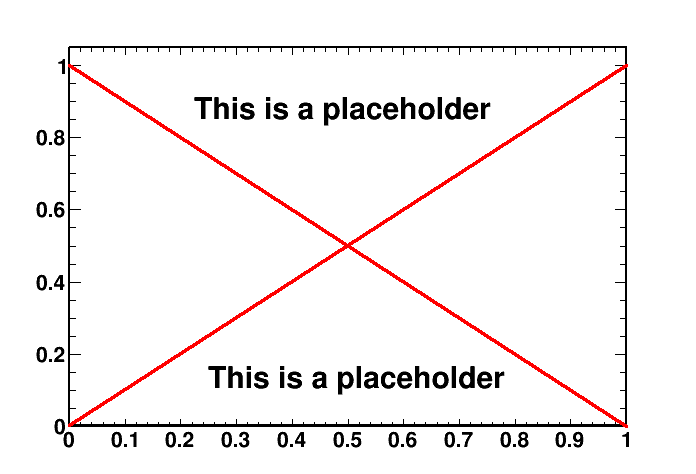
\includegraphics[width=.9\linewidth]{pic/dummy.png}
  \caption{Picture background only spectra with bad fit (high energies too hard) Compare bubble or disk region and outside}
  \label{fig:bkgd_only_spectrum}
\end{figure}

It can also be observed that the fit is particularly bad in the bubbles and the disk (see Fig. \ref{fig:original_GC_excess}) where the high energy spectrum is harder (see Fig. \ref{fig:bkgd_only_spectrum}). In this region, the PCR spectrum falls off too quickly, and the IC spectrum which usually takes care of high energies is blocked by the low energy flux drop.


%I was able to recreate a more or less spherical excess in GC around 2GeV.\\
%Bad fit in disk and bubbles as expected.
%Two problems :
%\begin{itemize}
%\item Spectrum too hard at high energies
%\item Excess around 2GeV
%\end{itemize}


\section{Introducing SCR}

\begin{figure}[h]
  	\centering
	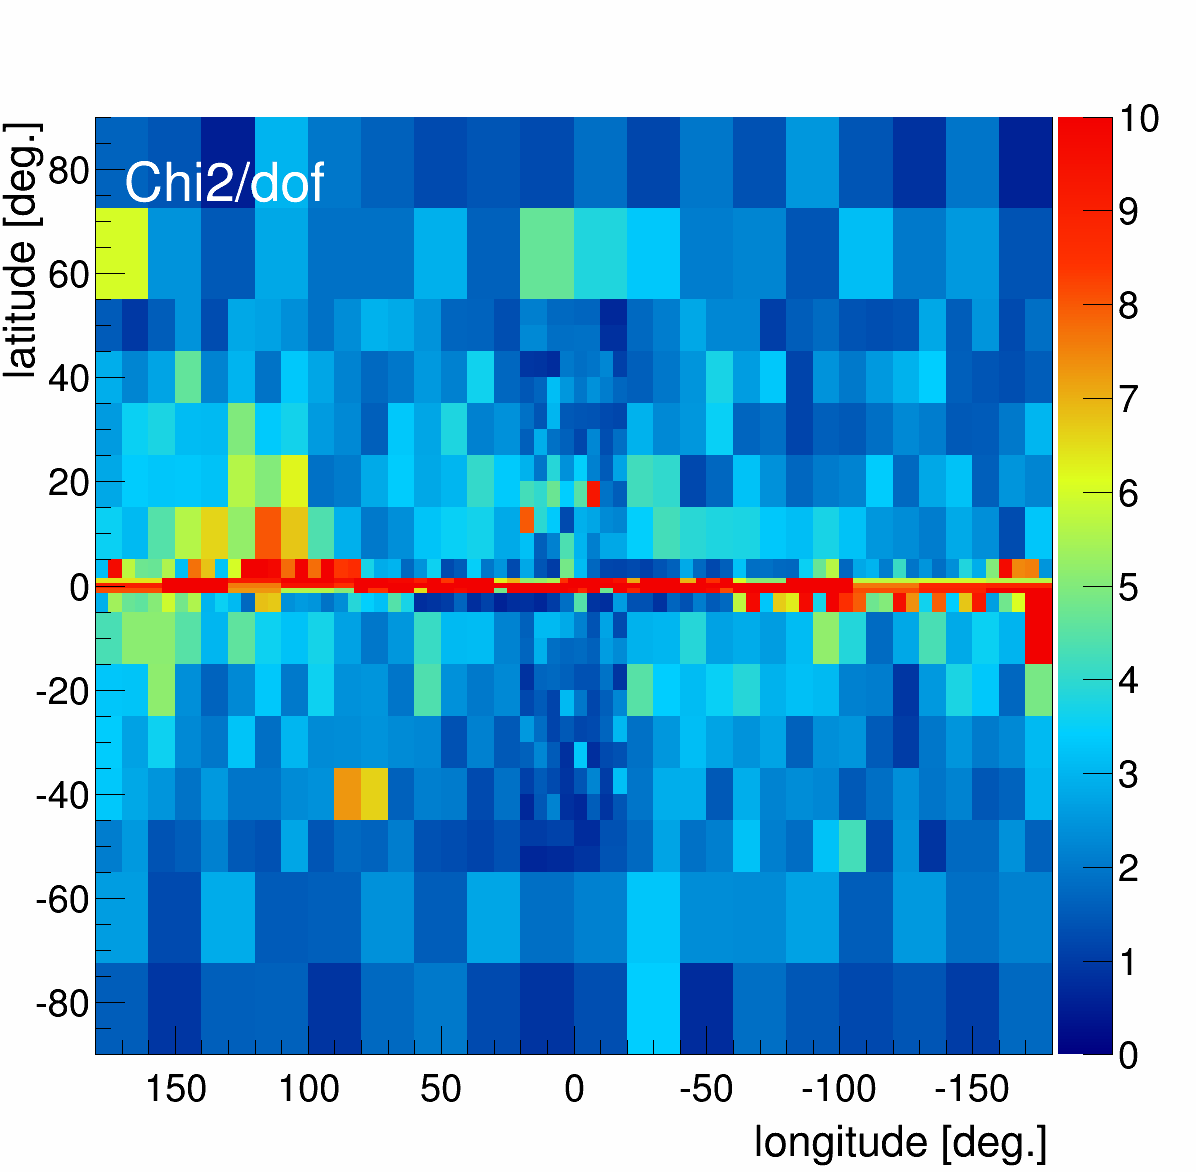
\includegraphics[width=.9\linewidth]{pic/results/SCRonly_Chi2Distribution.png}
  	\caption{Chi2 distribution of SCR only fits.}
  	\label{fig:SCRonly_fit}
\end{figure}

Introducing the SCR template, a clear improvement can be noted in the $\chi^2$ distribution (see Fig. \ref{fig:SCRonly_fit}). The bubble shape that was clear before has now disapeared. Even if the fit is still not perfect everywhere, the improvement is significant.

\begin{figure}[h]
  \centering
  \begin{minipage}[h]{0.45\textwidth}
  	\centering
	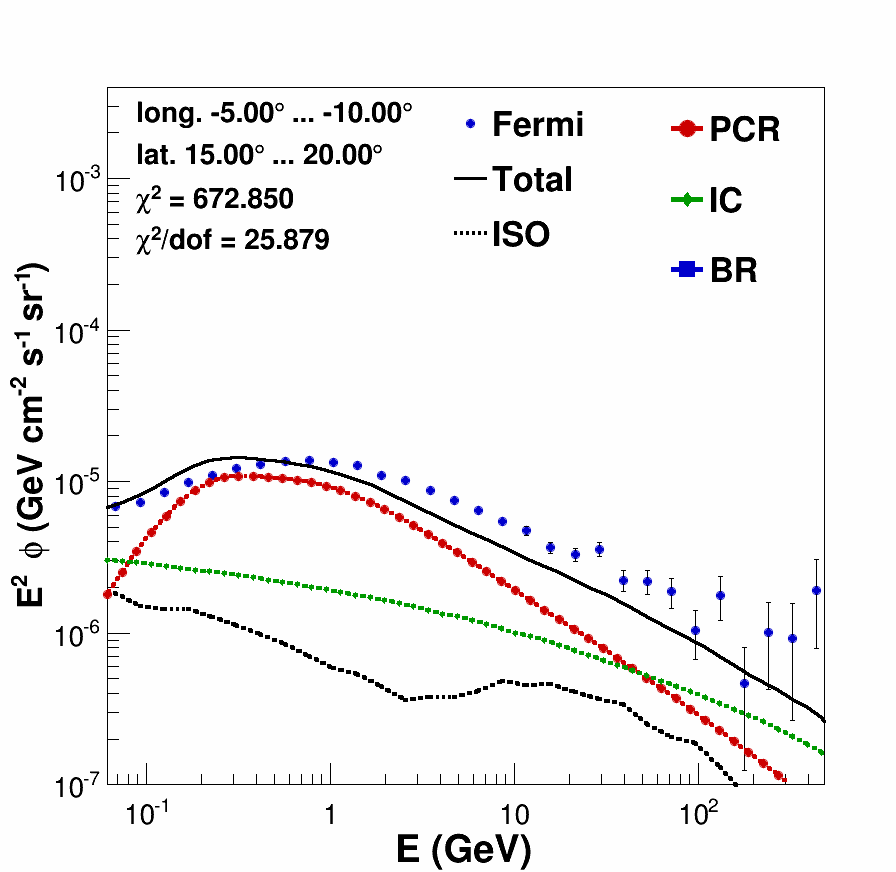
\includegraphics[width=1.\linewidth]{pic/results/bkgdonly_spectra_bubble_example.png}
  	\subcaption{Spectrum from a bubble with SCR only and background only.}
  	\label{fig:SCRonly_bubble_spec}
  \end{minipage}
  \hfill
  \begin{minipage}[h]{0.45\textwidth}
	  \centering
	  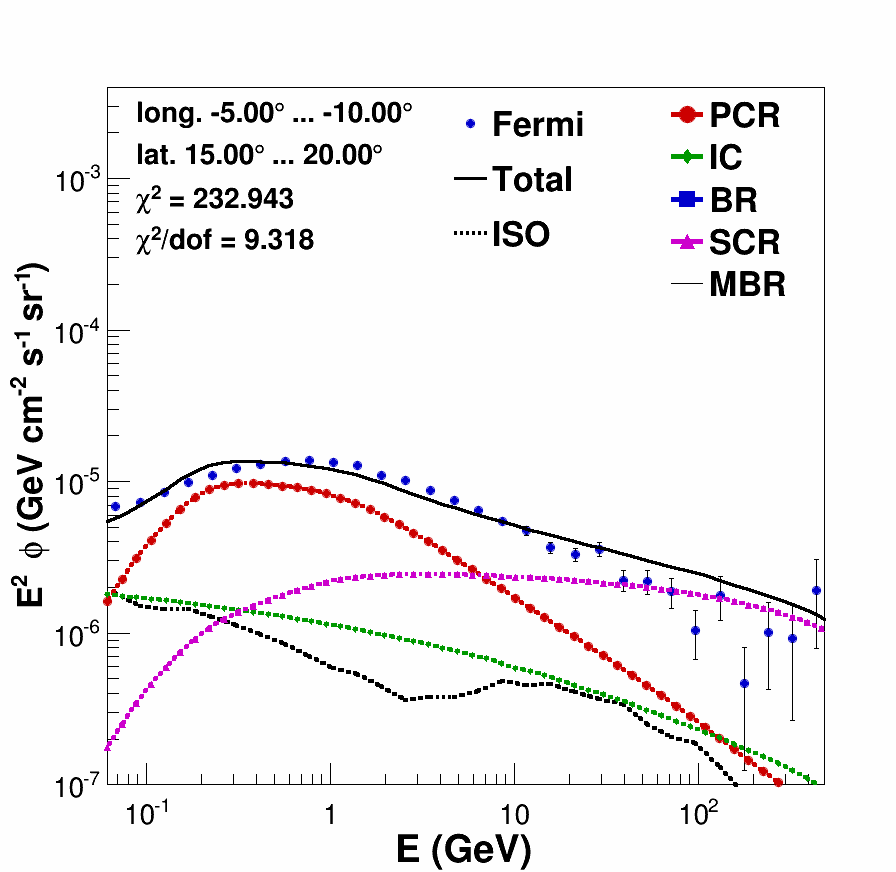
\includegraphics[width=1.\linewidth]{pic/results/SCRonly_spectra_bubble_example.png}
	  \subcaption{Spectrum from a bubble with background models only and background only.}
	  \label{fig:BKGonly_bubble_spec}
  \end{minipage}	 
\end{figure}

From Fig. \ref{fig:SCRonly_bubble_spec} and \ref{fig:SCRonly_bubble_spec} we see the role of the SCR template at high energies, taking care of the high flux. It also permits a better fit of low energies by PCR and IC since they do not have to be everywhere at the same time.

\todo{Here the bad chi2 comes from 0.1GeV region, where the PCR template does not fit the data. not from the 2GeV excess.}
A problem still remains in the disk and diffuse regions around the galactic anticenter. 



\section{Introducing SCR and MCR}
%	-Introduction of SCR and MCR
%		-very good chi2 in disk and bubbles
%		-spatial shapes of comps
%			-IC sperical (as expected) but depletion in disk
%			-BR low in bubbles replaces IC in disk
%			-PCR OK but low in disk
%			-MCR follows CO map, take place of PCR in disk
%			-SCR follows bubble structure

\begin{figure}[h]
  \centering
%   \todo{May have to change it if we change the bckground model} 
  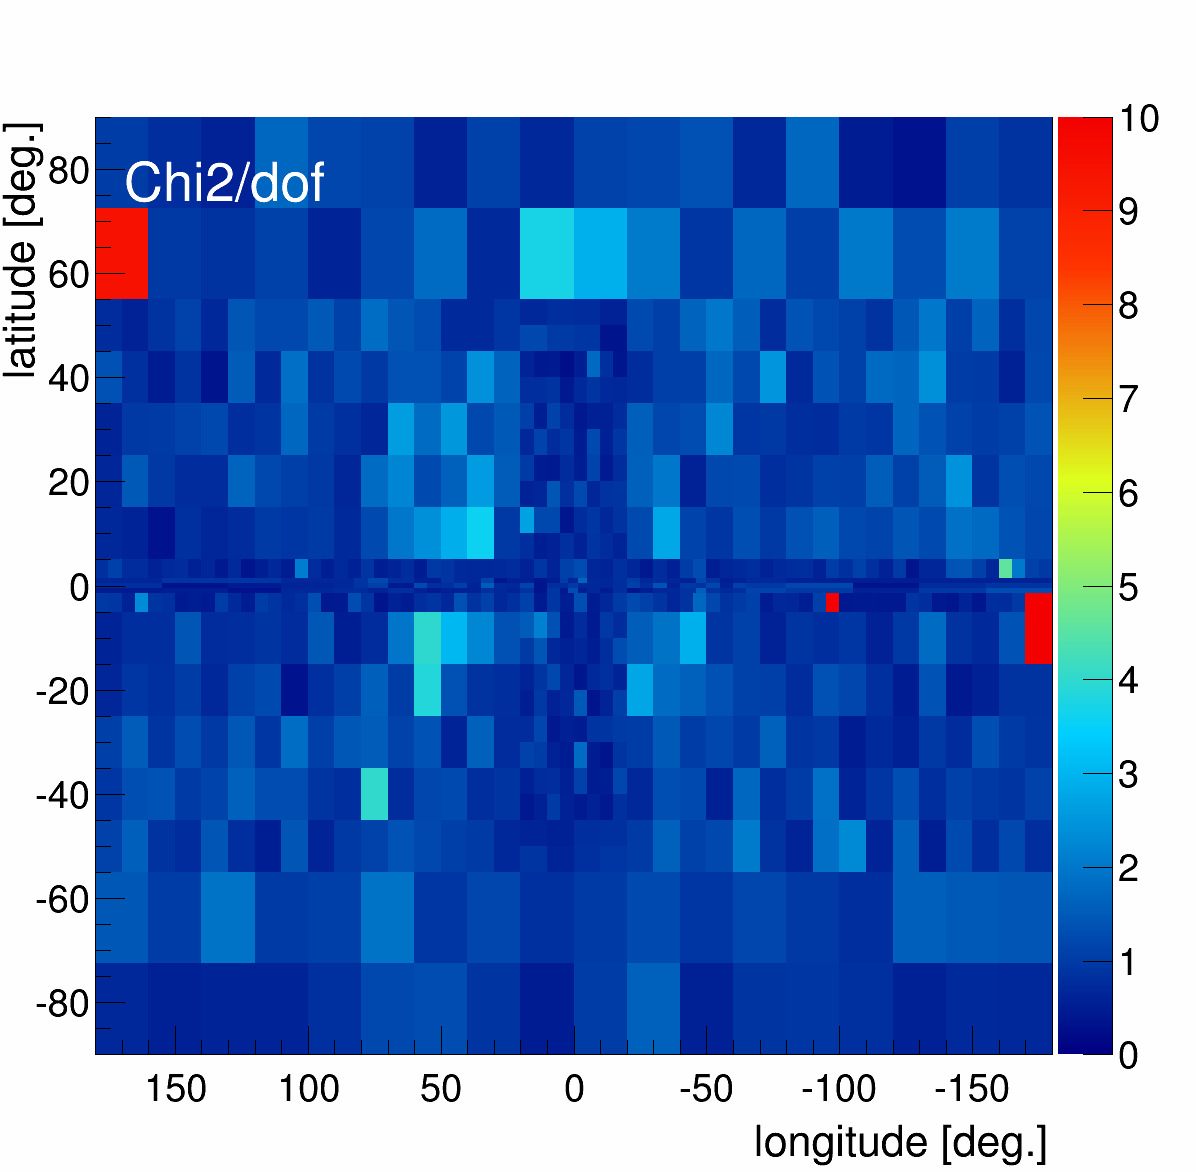
\includegraphics[width=.9\linewidth]{pic/results/MCRonly_chi2Distribution.png}
  \caption{Chi2 maps of MCRonly fits compared to background only}
  \label{fig:MCRonly_chi2Distribution}
\end{figure}
%First obvious thing is the good chi2 in the disk and bubbles.\\

As shown on Fig. \ref{fig:MCRonly_chi2Distribution}, the addition of a new template improve significantly the $\chi^2$ distribution in all directions. The bubbles and the disk structures are not visible anymore.

Three dots appear to have a really high $\chi^2$, but that is only due to the point source subtraction that is not perfect (see Chapt. \ref{sec:Data_origin}).

\begin{figure}[h]
  \centering
  
  \begin{minipage}[h]{0.45\textwidth}
	  \centering
	  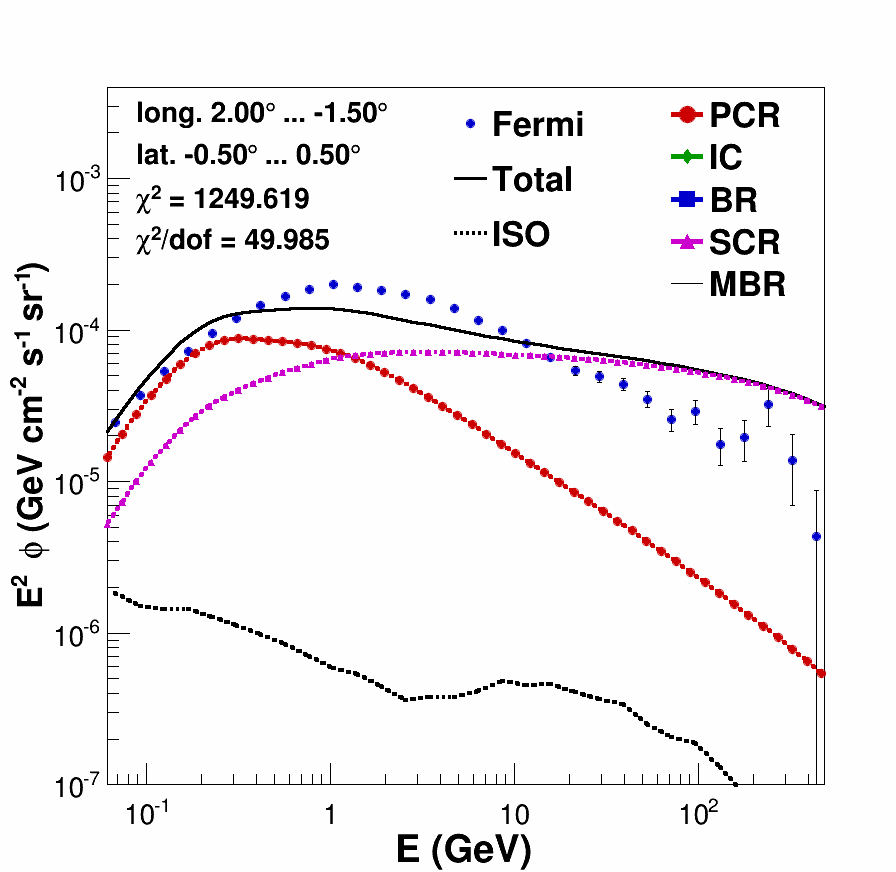
\includegraphics[width=\linewidth]{pic/results/SCRonly_CMZ.png}	  
  	  \subcaption{SCR fit in the CMZ region}
	  \label{fig:SCRonly_CMZ}
  \end{minipage}
  \hfill
  \begin{minipage}[h]{0.45\textwidth}
	  \centering
	  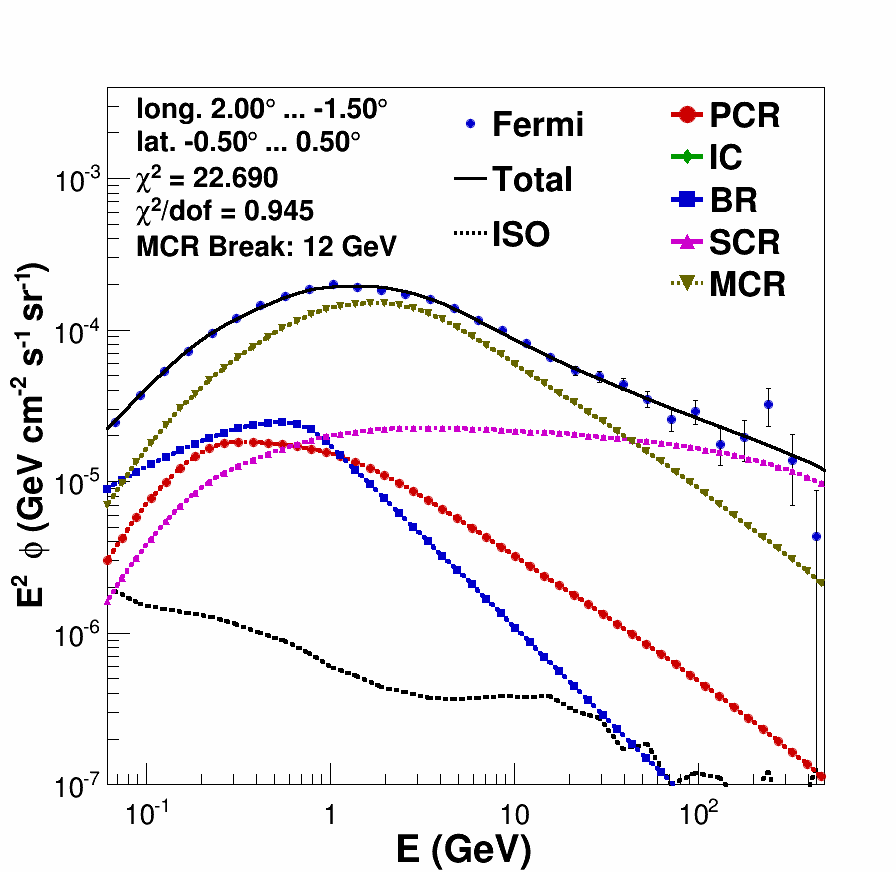
\includegraphics[width=\linewidth]{pic/results/MCRonly_CMZ.png}
	  \subcaption{MCR fit in the CMZ region}
  	  \label{fig:MCRonly_CMZ}
  \end{minipage}
  \label{fig:MCR_vs_SCRonly_CMZ}
\end{figure}

Fig. \ref{fig:MCR_vs_SCRonly_CMZ} shows the central molecular zone (CMZ) fitted with and without the MCR component. The gas density is very high in this region, hence it is the first region where we would expect the MCR emission to be present, if not dominant compared to PCR. Indeed the fit chooses this configuration, with the MCR template dominating all the others and we can directly see the improvement in the MCR fit. The energies around 2GeV had a clear excess that the four components of the SCR fit could not account for. The MCR template peaking in this region, it comes in very handy and fill this gap, Leaving the SCR template taking care of the high energies and PCR and BR for the low energies. \todo{Why isn't there IC? -> Wait to see if we change the models}



\subsection{Discussion on spatial shapes}
\begin{figure}
  \centering
  \begin{minipage}[h]{0.45\textwidth}
  	\centering
	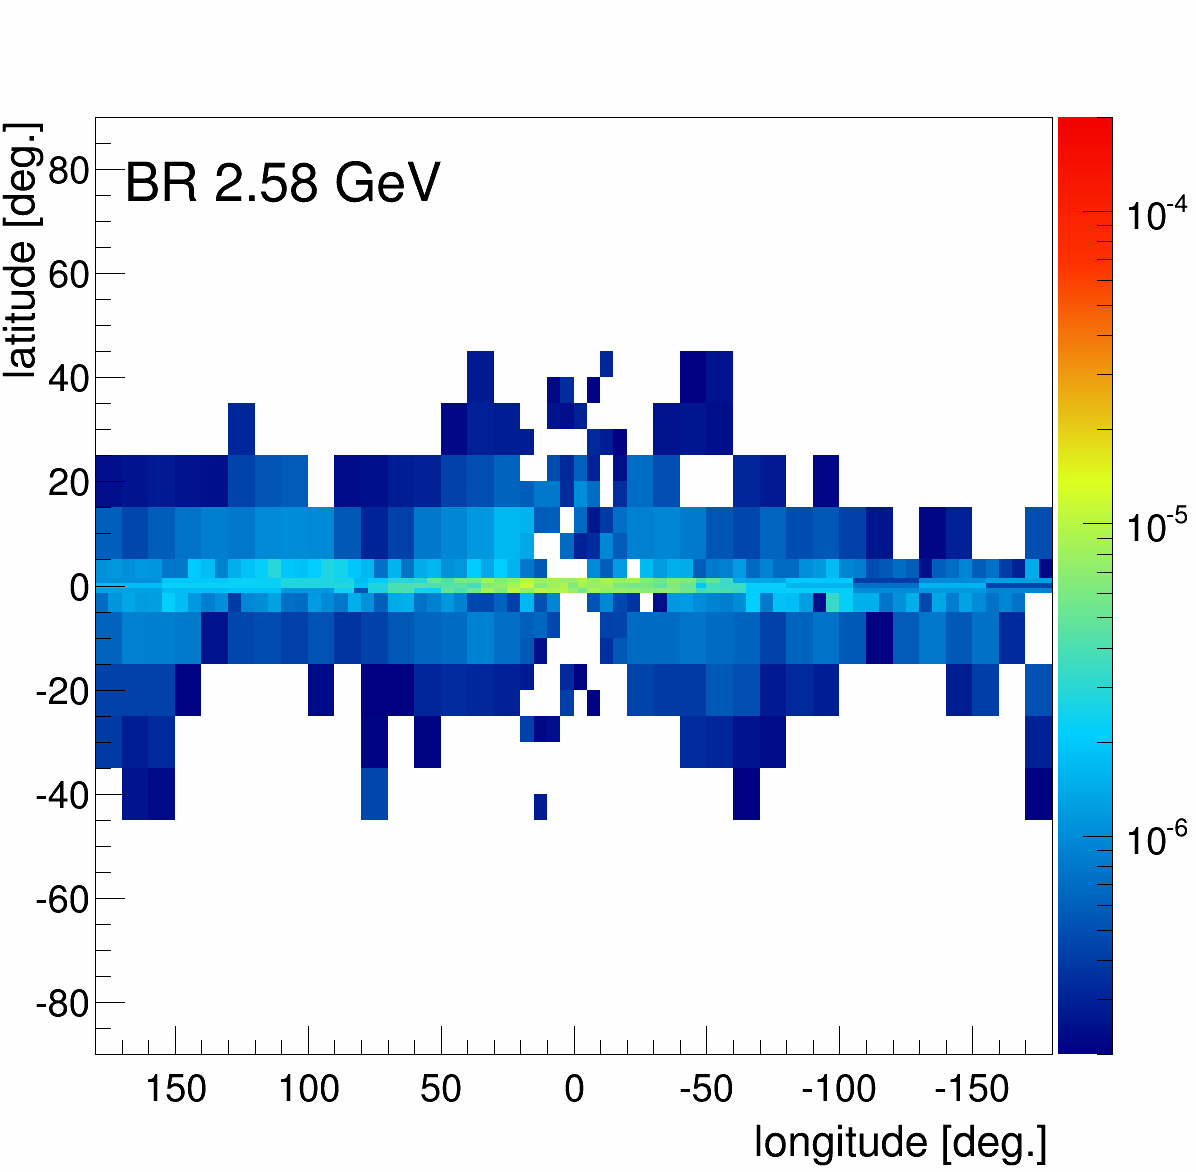
\includegraphics[width=1.\linewidth]{pic/results/MCRonly_BR_fluxE12_skymap.png}
  	\subcaption{Flux distribution of bremstrahlung (BR)}
  	\label{fig:MCRonly_skymap_BR}
  \end{minipage}
  \hfill
  \begin{minipage}[h]{0.45\textwidth}
  	\centering
	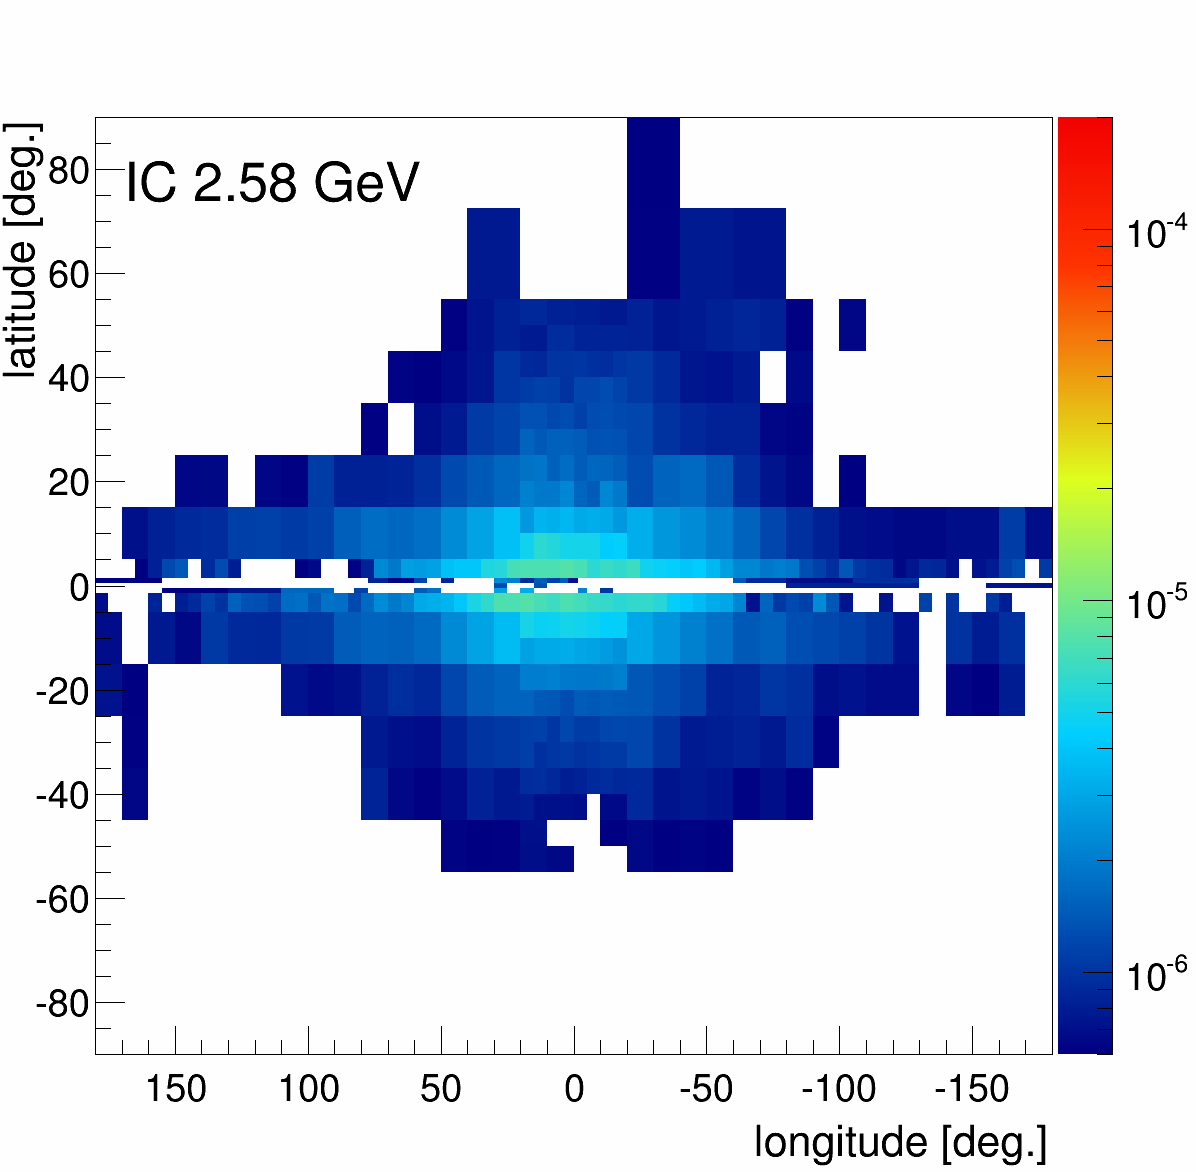
\includegraphics[width=1.\linewidth]{pic/results/MCRonly_IC_fluxE12_skymap.png}
  	\subcaption{Flux distribution of inverse compton (IC)}
  	\label{fig:MCRonly_skymap_IC}
  \end{minipage}
  \hfill
  \begin{minipage}[h]{0.45\textwidth}
  	\centering
	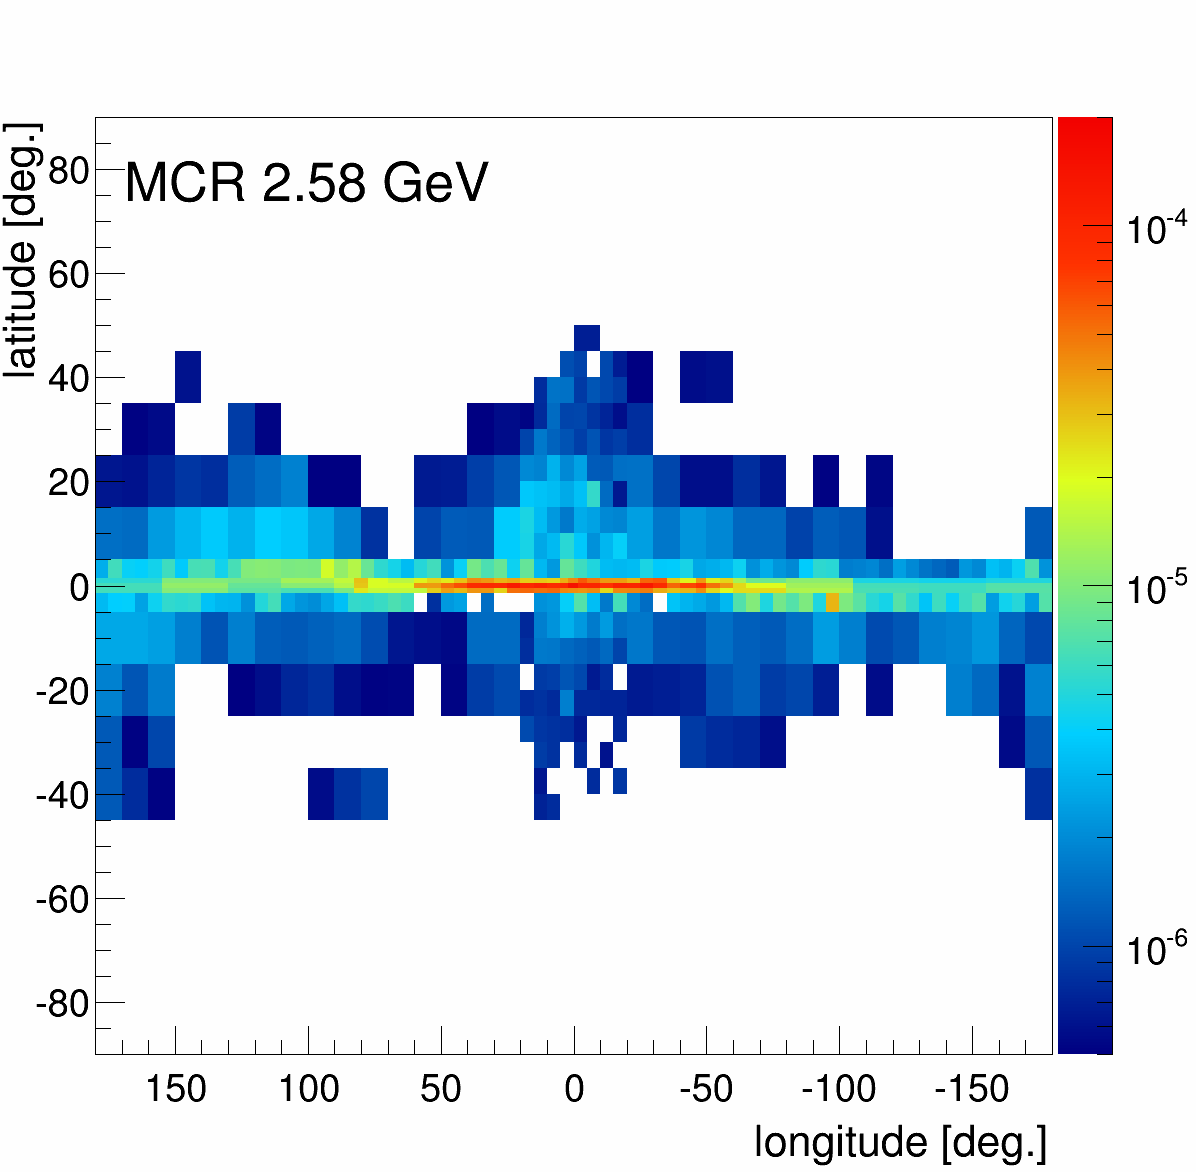
\includegraphics[width=1.\linewidth]{pic/results/MCRonly_MCR_fluxE12_skymap.png}
  	\subcaption{Flux distribution of MCR}
  	\label{fig:MCRonly_skymap_MCR}
  \end{minipage}
  \hfill
  \begin{minipage}[h]{0.45\textwidth}
  	\centering
	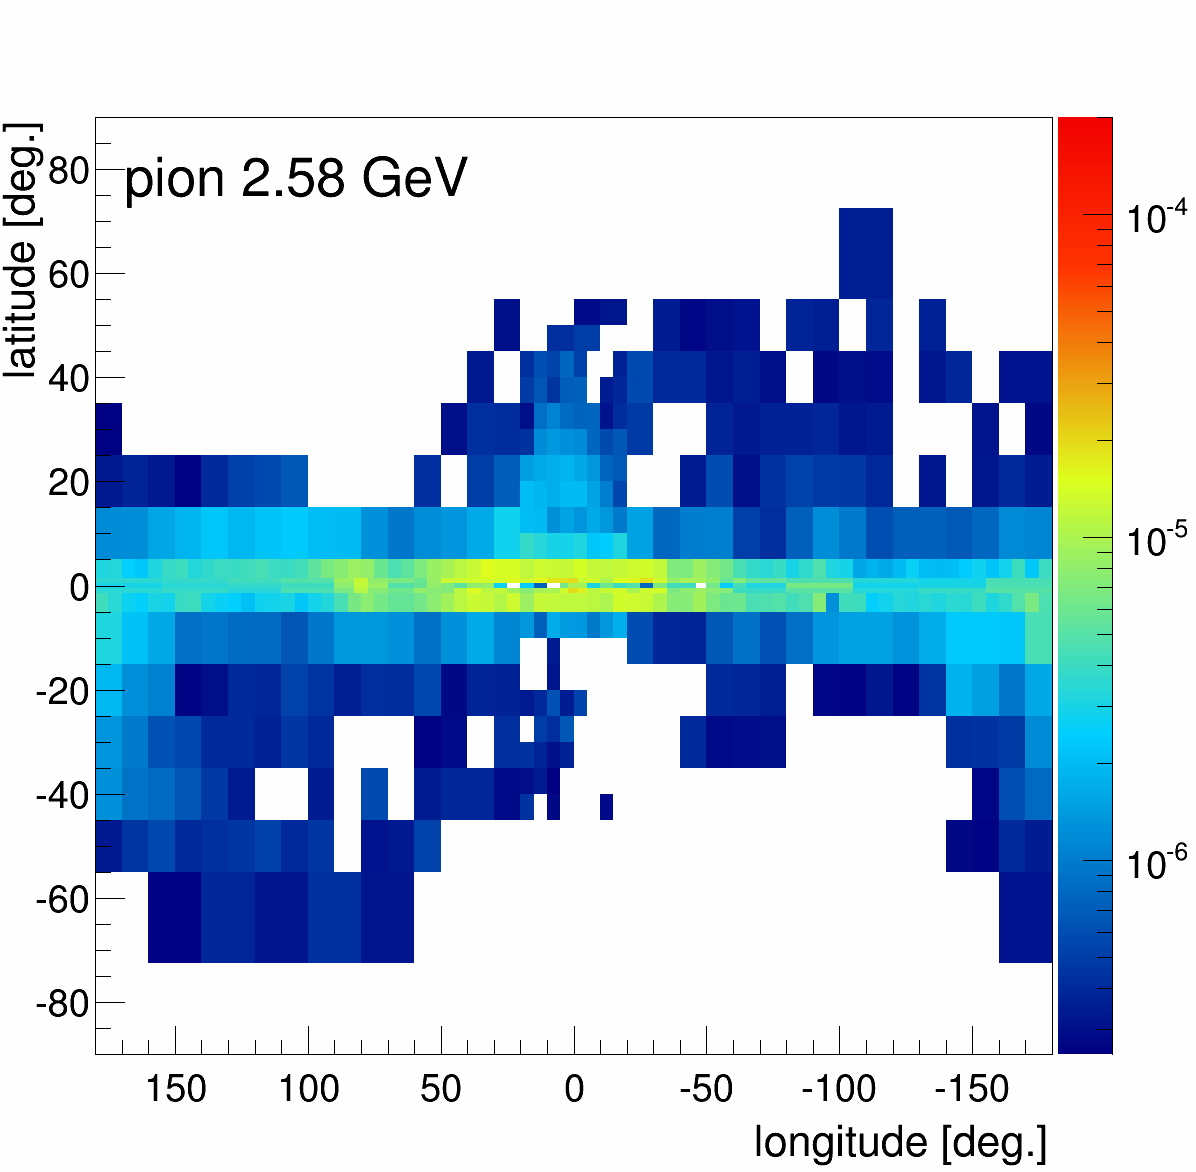
\includegraphics[width=1.\linewidth]{pic/results/MCRonly_PCR_fluxE12_skymap.png}
  	\subcaption{Flux distribution of PCR}
  	\label{fig:MCRonly_skymap_PCR}
  \end{minipage}
  \hfill
  \begin{minipage}[h]{0.45\textwidth}
  	\centering
	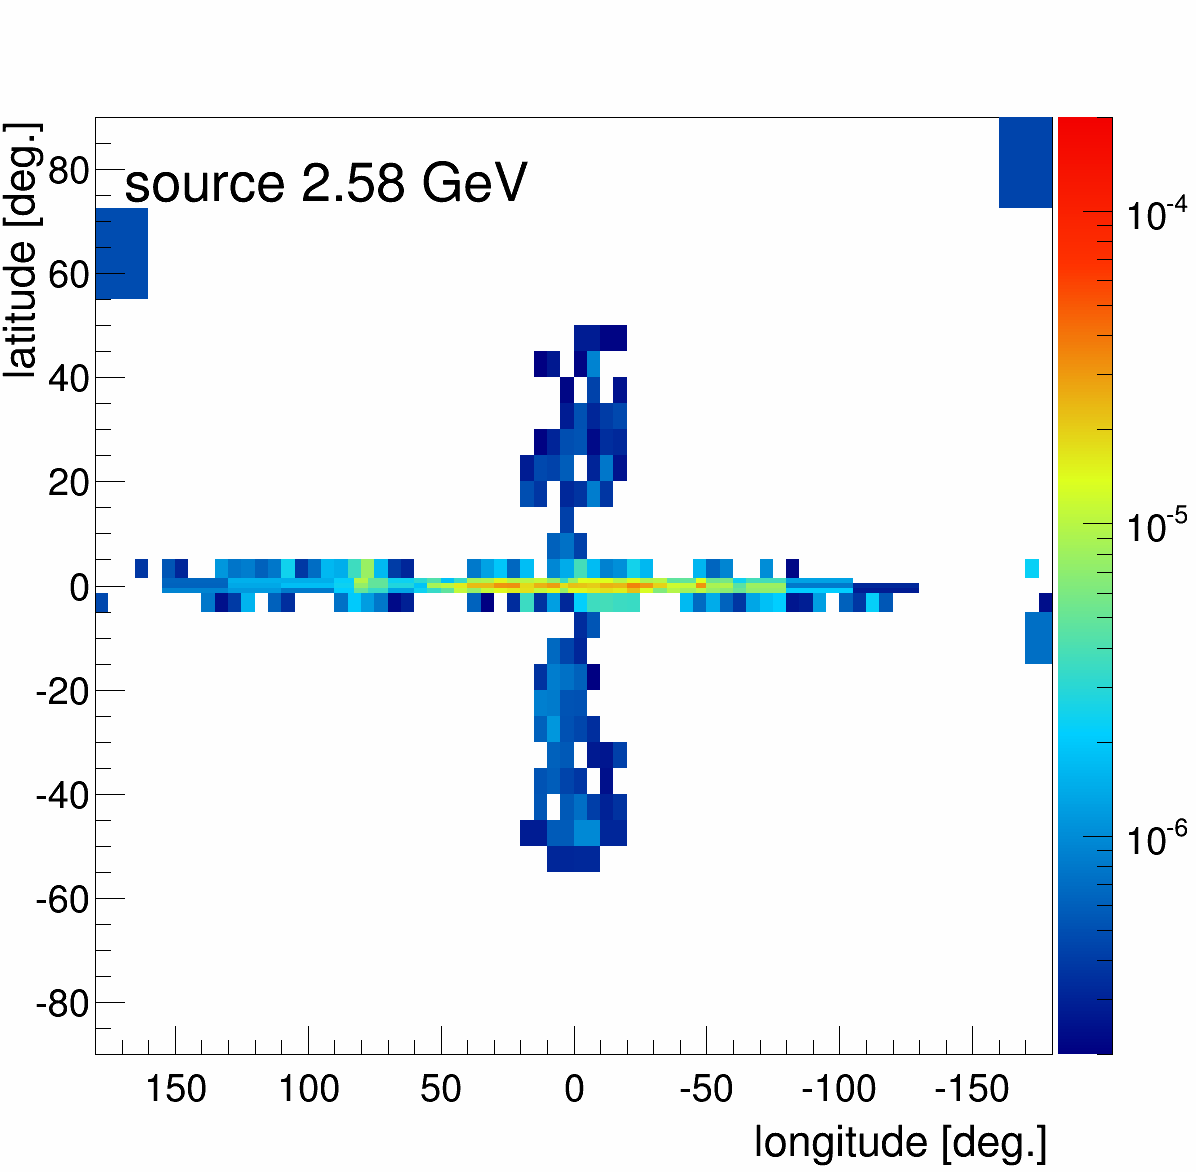
\includegraphics[width=1.\linewidth]{pic/results/MCRonly_SCR_fluxE12_skymap.png}
  	\subcaption{Flux distribution of SCR}
  	\label{fig:MCRonly_skymap_SCR}
  \end{minipage}
  \hfill
  \begin{minipage}[h]{0.45\textwidth}
  	\centering
	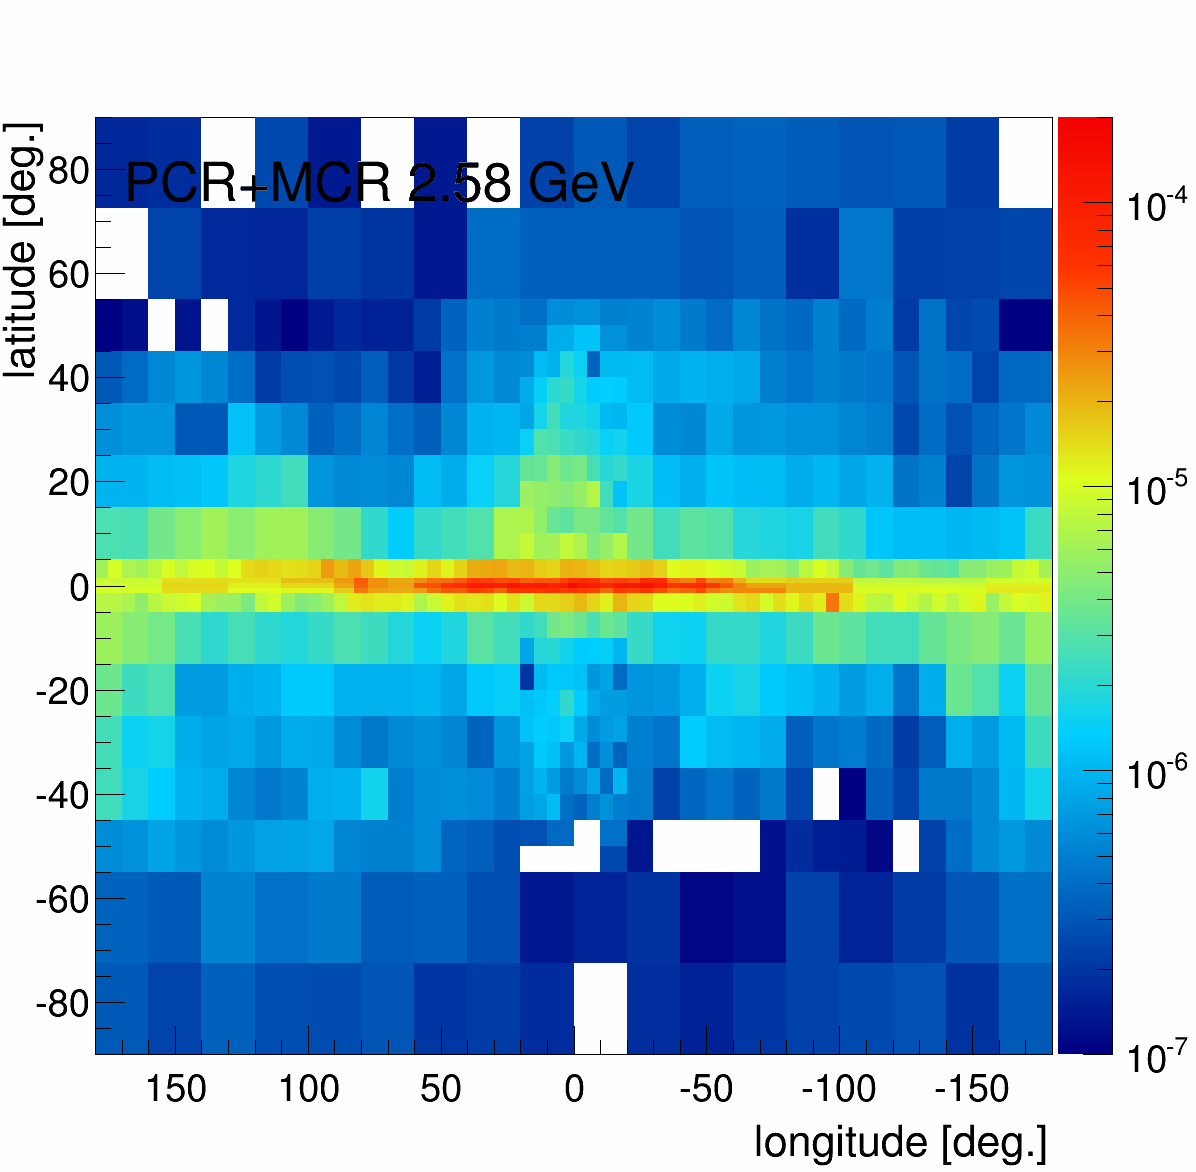
\includegraphics[width=1.\linewidth]{pic/results/MCRonly_PCR+MCR_fluxE12_skymap.png}
  	\subcaption{Flux distribution of PCR + MCR}
  	\label{fig:MCRonly_skymap_PCR+MCR}
  \end{minipage}
  \label{fig:MCRonly_skymaps}
\end{figure}

Fig. \ref{fig:MCRonly_skymaps} shows the spatial distribution of the flux of each component around 2GeV, as returned by the fit.

The bremmstrahlung component is consistent with the the expectations. Present everywhere, it is strong in the disk, and decrease a little in the bubbles.

Though the general shape is sperical, the IC component has an unexpected feature in the form of a strong depletion in the disk, like a "sandwich" structure. This is surprising in the sense that this is where the interstellar radiation field (ISRF) and electron density are supposed to be maximal, creating a higher IC flux. A possible explanation could be coming from the dust distribution, screening the starlight component of the ISRF. Thus depriving the ISRF of its main component and leaving only the dust infra red emission and the CMB to interact with the electrons. This could result in a lower IC gamma-ray flux in the disk.

The SCR component is playing his role perfectly, filling the bubbles and the disk, where the high energy portion of the spectra needs a harder spectrum. It traces perfectly the sources distribution in the disk and the outflow of high energy protons in the bubbles.

The general shape of PCR looks coherent with he shape of the galaxy, with a strong flux in the bar and the galactic disk in general. When looking closely, one can see the same kind of depletion in the disk than for IC, even if the effect is less remarkable. This finds its cause in the MCR distribution with a very high flux in the disk. The sum of both templates (MCR + PCR) shows no sign of such a feature, which tends to show that some of the PCR photons are absorbed by the MCR template. But the total is coherent, with no unexplainable central gap.

The MCR template also follows the spatial distribution of molecular clouds in our galaxy. It is a good sign since it is supposed to come from those regions.
It is not spherical at all. That could have happened if the excess component has a DM origin, since it is supposed to be spherically distributed.


\section{Introducing SCR and DM}
%	-Introduction of SCR + DM
%		-chi2
%		-spatial shapes	
%		-Weniger plots
%		-Specklings

\begin{figure}
  \centering
  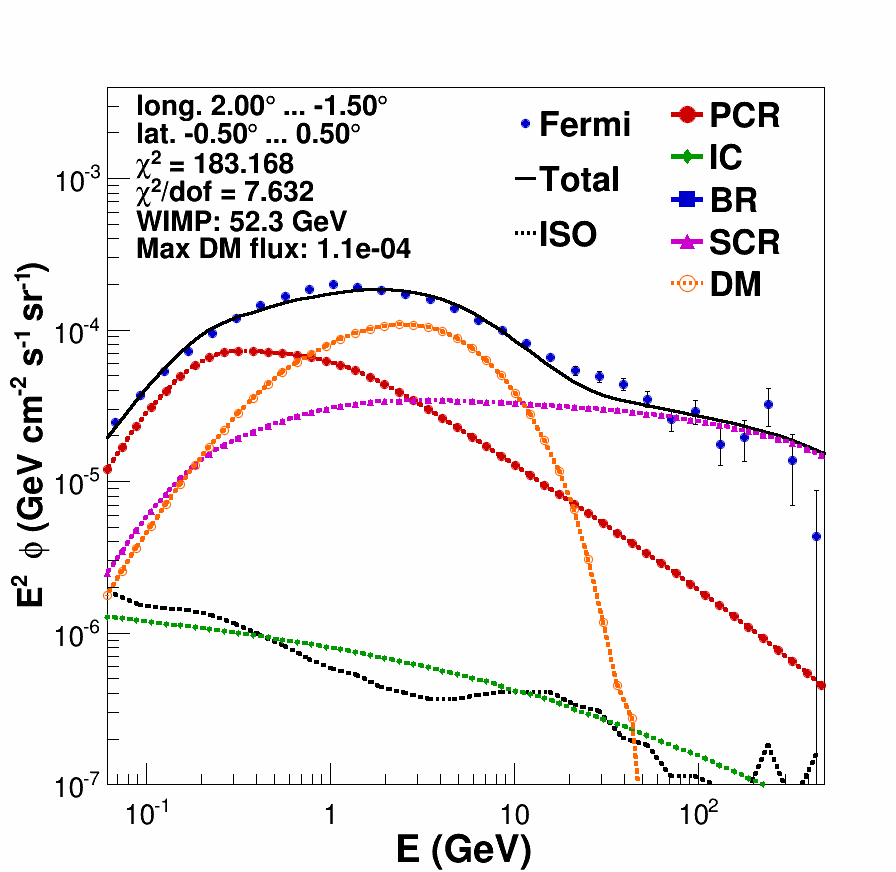
\includegraphics[width=.9\linewidth]{pic/results/DMonly_CMZ.png}
  \caption{spectrum of best mass DM fitted in CMZ. Also pictures of DM distribution compared to gas map.}
  \label{fig:DMonly_CMZ}
\end{figure}

\begin{figure}
  \centering
  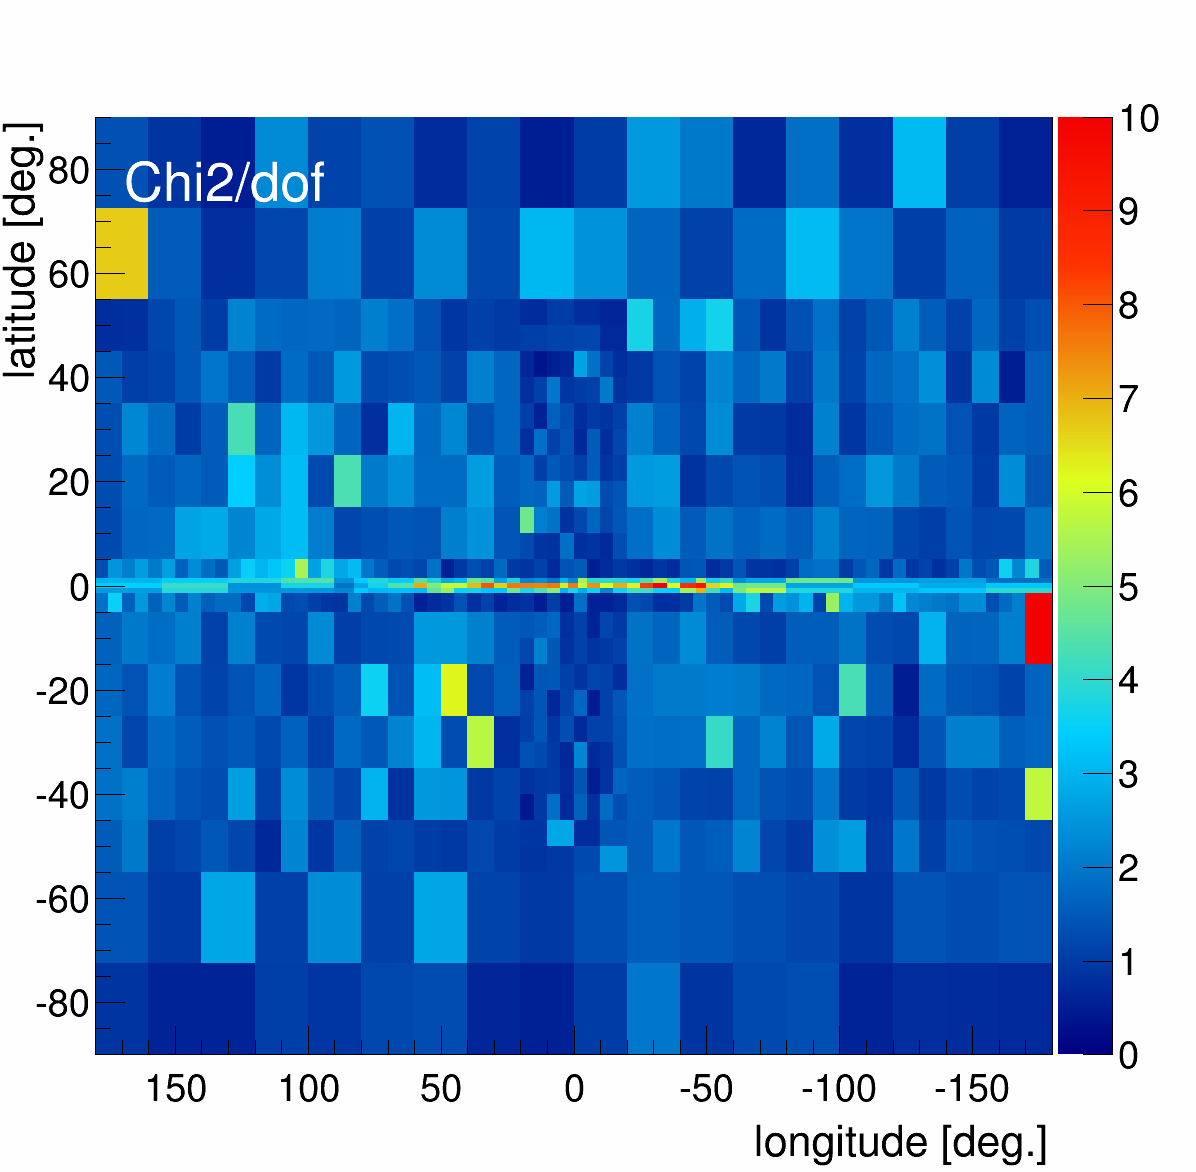
\includegraphics[width=.9\linewidth]{pic/results/DMonly_chi2Distribution.png}
  \caption{DM fit chi2 distribution}
  \label{fig:DMonly_chi2Distribution}
\end{figure}

\begin{figure}
  \centering
  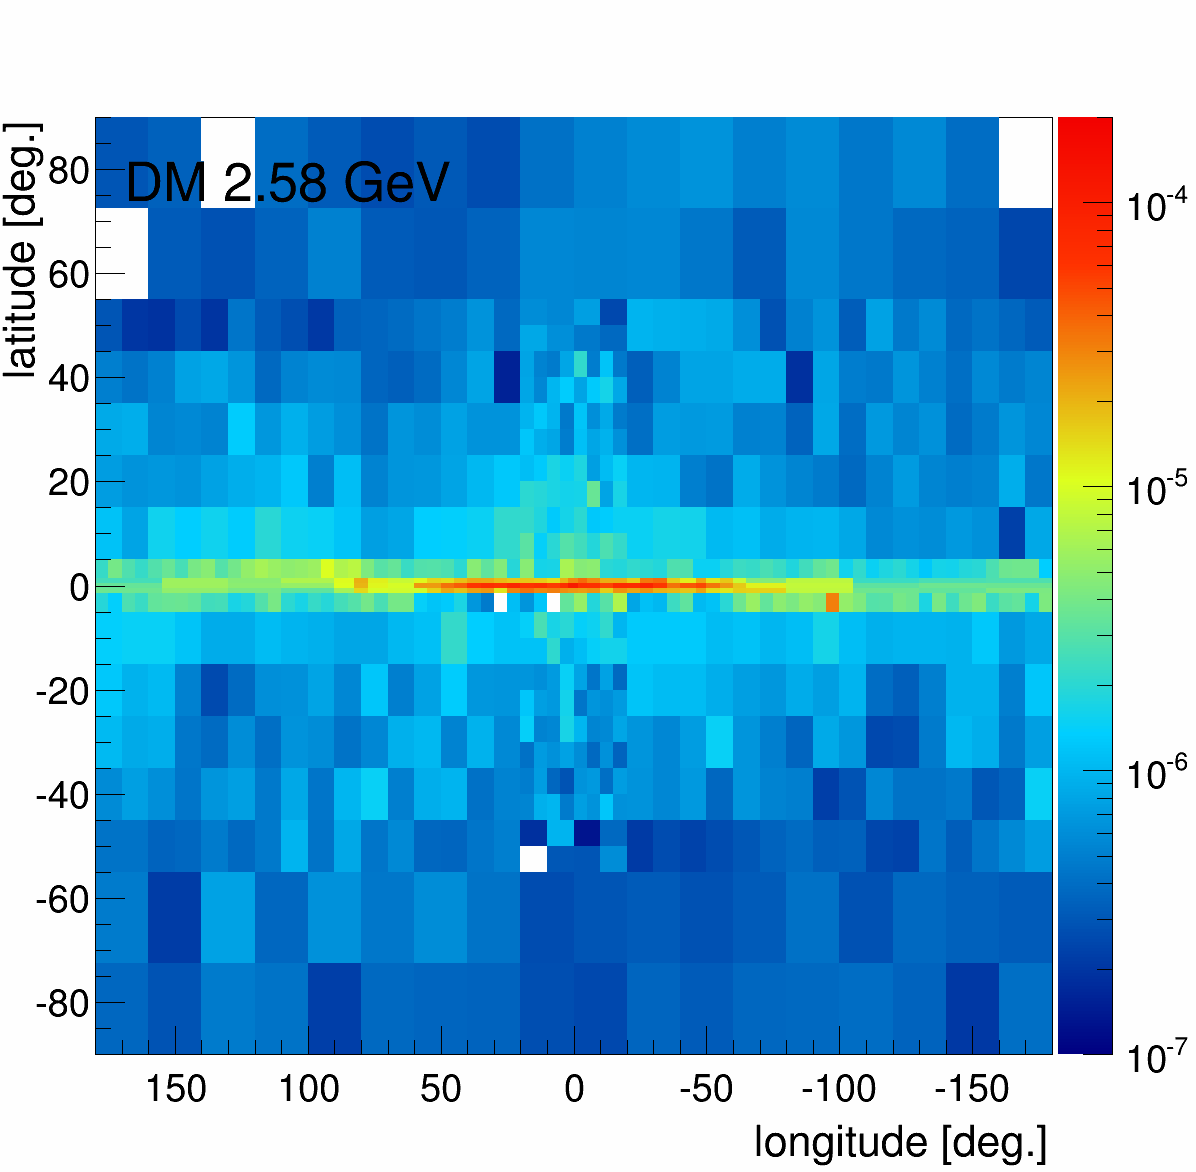
\includegraphics[width=.9\linewidth]{pic/results/DMonly_DM_fluxE12_skymap.png}
  \caption{DM distribution compared to gas map.}
  \label{fig:DMonly_skymap_DM}
\end{figure}


The first step is to determine which mass for the WIMP particles would produce the best spectrum for our fit. Fig. \ref{fig:DMonly_CMZ} shows the best fit for the CMZ region, with the WIMP mass as a free parameter. It chooses a mass of 52.3 GeV, peaking around a few GeV, as expected in \todo{ref theory section}. Since the excess is the most significant in this region, it is also the best place to define our mass for the rest of the sky. This is what is done in the following section.


Once the mass is determined for the entire sky, the fit gives the following results. The $\chi^2$ distribution (Fig. \ref{fig:DMonly_chi2Distribution} is comparable to the MCR fit for the major part but is significantly worst in the disk.


As seen on Fig. \ref{fig:DMonly_skymap_DM}, the DM distribution of the fit traces closely the distribution of molecular gas distribution (as traced by CO).



\section{Introducing SCR and MSP}
%	-Introduction of SCR + MSP:
%		-chi2
%		-spatial shapes
%		-Weniger plots
%		-Specklings

\begin{figure}
  \centering
  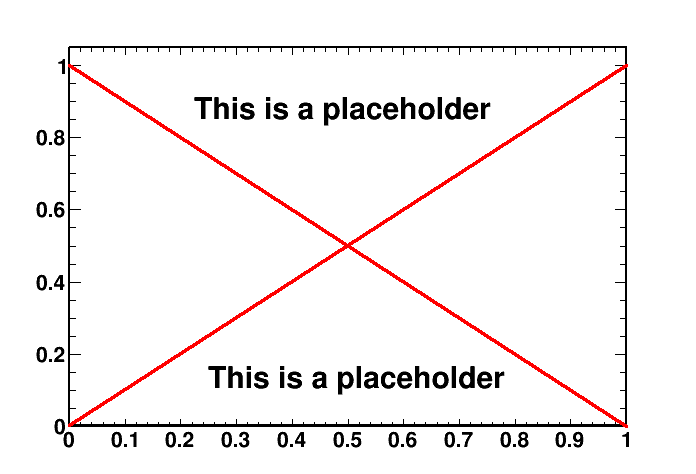
\includegraphics[width=.9\linewidth]{pic/dummy.png}
  \caption{pictures of MSP spectrum, chi2. Residuals at low energy maybe?}
  \label{fig:MSPonly_fit}
\end{figure}

Bad chi2 compared to MCR. The low energy spectrum is too hard.






